\problemname{Bílskúrar}
\illustration{0.3}{garage}{Mynd fengin af \href{https://upload.wikimedia.org/wikipedia/commons/d/d0/Garage\%2C_Hovslagargatan\%2C_V\%C3\%A4nersborg.jpg}{wikimedia.org}}

Hannes býr í Brúnalandi.
Í Brúnalandi er aðeins ein gata og eru öll húsin öðrum megin við götuna.
Hinum megin við götuna eru bílskúrarnir.
Hvert hús er með númer og hver bílskúr er einnig með númer.
Eigandi hús á þá einnig bílskúrinn með sama númeri.

Eðlilegast væri að húsin væru númeruð í hækkandi röð 
og að bílskúr hvers húss væri beint á móti húsinu.
Brúnaland var hins vegar ekki planað mjög vel og er röð húsanna og bílskúranna í algjöru rugli.

Þegar húseigendur ferðast milli húss og bílskúrs ferðast þeir eftir beinni línu.
Þetta getur skapað marga árekstra þegar fólk er að ferðast milli húsa og bílskúra sinna.
Hversu mörg pör húseigenda geta mögulega lent í árekstri á leið í bílskúrana sína.


\section*{Inntak}
Fyrsta línan í inntakinu inniheldur eina heiltölu $n$ ($1 \leq n \leq
2\cdot10^5$), fjöldi húsa í götunni.
Önnur línan inniheldur $n$ heiltölur, sem lýsa í hvaða röð húsin eru. Hver tala á bilinu $1$ upp í $n$ kemur fyrir nákvæmlega einu sinni.
Þriðja línan inniheldur $n$ heiltölur, sem lýsa í hvaða röð bílskúrarnir eru. Hver tala á bilinu $1$ upp í $n$ kemur fyrir nákvæmlega einu sinni.

\section*{Úttak}
Skrifaðu út eina heiltölu, fjölda árekstra sem gætu átt sér stað.

\section*{Útskýring á sýnidæmi}
Fyrsta sýnidæmið fellur undir hóp 3. Þar má sjá leiðirnar sem húseigendurnir ganga frá húsum
að bílskúrum og alla mögulega árekstra sem gætu átt sér stað, merktir með fylltum rauðum hringjum.
\begin{figure}[h!]
  \centering
    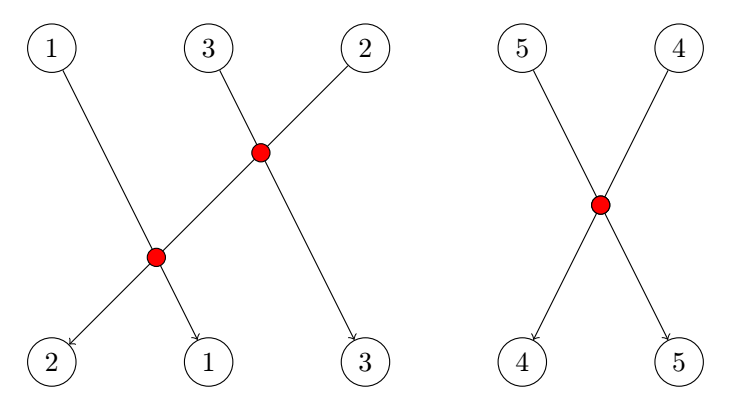
\includegraphics[width=0.5\textwidth]{sample_illustration}
  \caption{Sýnidæmi 1}
\end{figure}

\section*{Stigagjöf}
\begin{tabular}{|l|l|l|}
\hline
Hópur & Stig & Takmarkanir \\ \hline
1     & 20   & $1 \leq n \leq 10$ og húsnúmerin eru í hækkandi röð\\ \hline
2     & 20   & $1 \leq n \leq 10^3$ og húsnúmerin eru í hækkandi röð\\ \hline
3     & 20   & $1 \leq n \leq 10^3$\\ \hline
4     & 20   & Húsnúmerin eru í hækkandi röð\\ \hline
5     & 20   & Engar frekari takmarkanir\\ \hline
\end{tabular}

